\subsection{Physics at hadronic collision}
\label{hadroniccollision}

Protons are not the elementary particle, which actually be composed of quarks and gluons.
So in proton-proton (pp) collision at the LHC, it is not protons themselves interact but quarks and gluons.
Scattering processes can then be further classified into either \textit{hard} or \textit{soft} processes
according to the momentum transfer during the interaction \cite{Dremin:2005wd}.
QCD, as an underlying theory for both two process, its approach and level of understandings in two cases are quite different.
For hard process, eg. Higgs, vector bosons and jets production, the rates and event
properties can be precisely predicted based on perturbation theory.
However, for soft processes like total cross-section, the underlying events, the rates and properties are dominated by non-perturbative QCD effects
that are less understood.
For many hard processes, the hard interactions are accompanied by soft ones.
A example of the hadronic collision is illustrated in figure~\ref{fig:C2_had_col}. 
\begin{figure}[!htb]
  \centering
  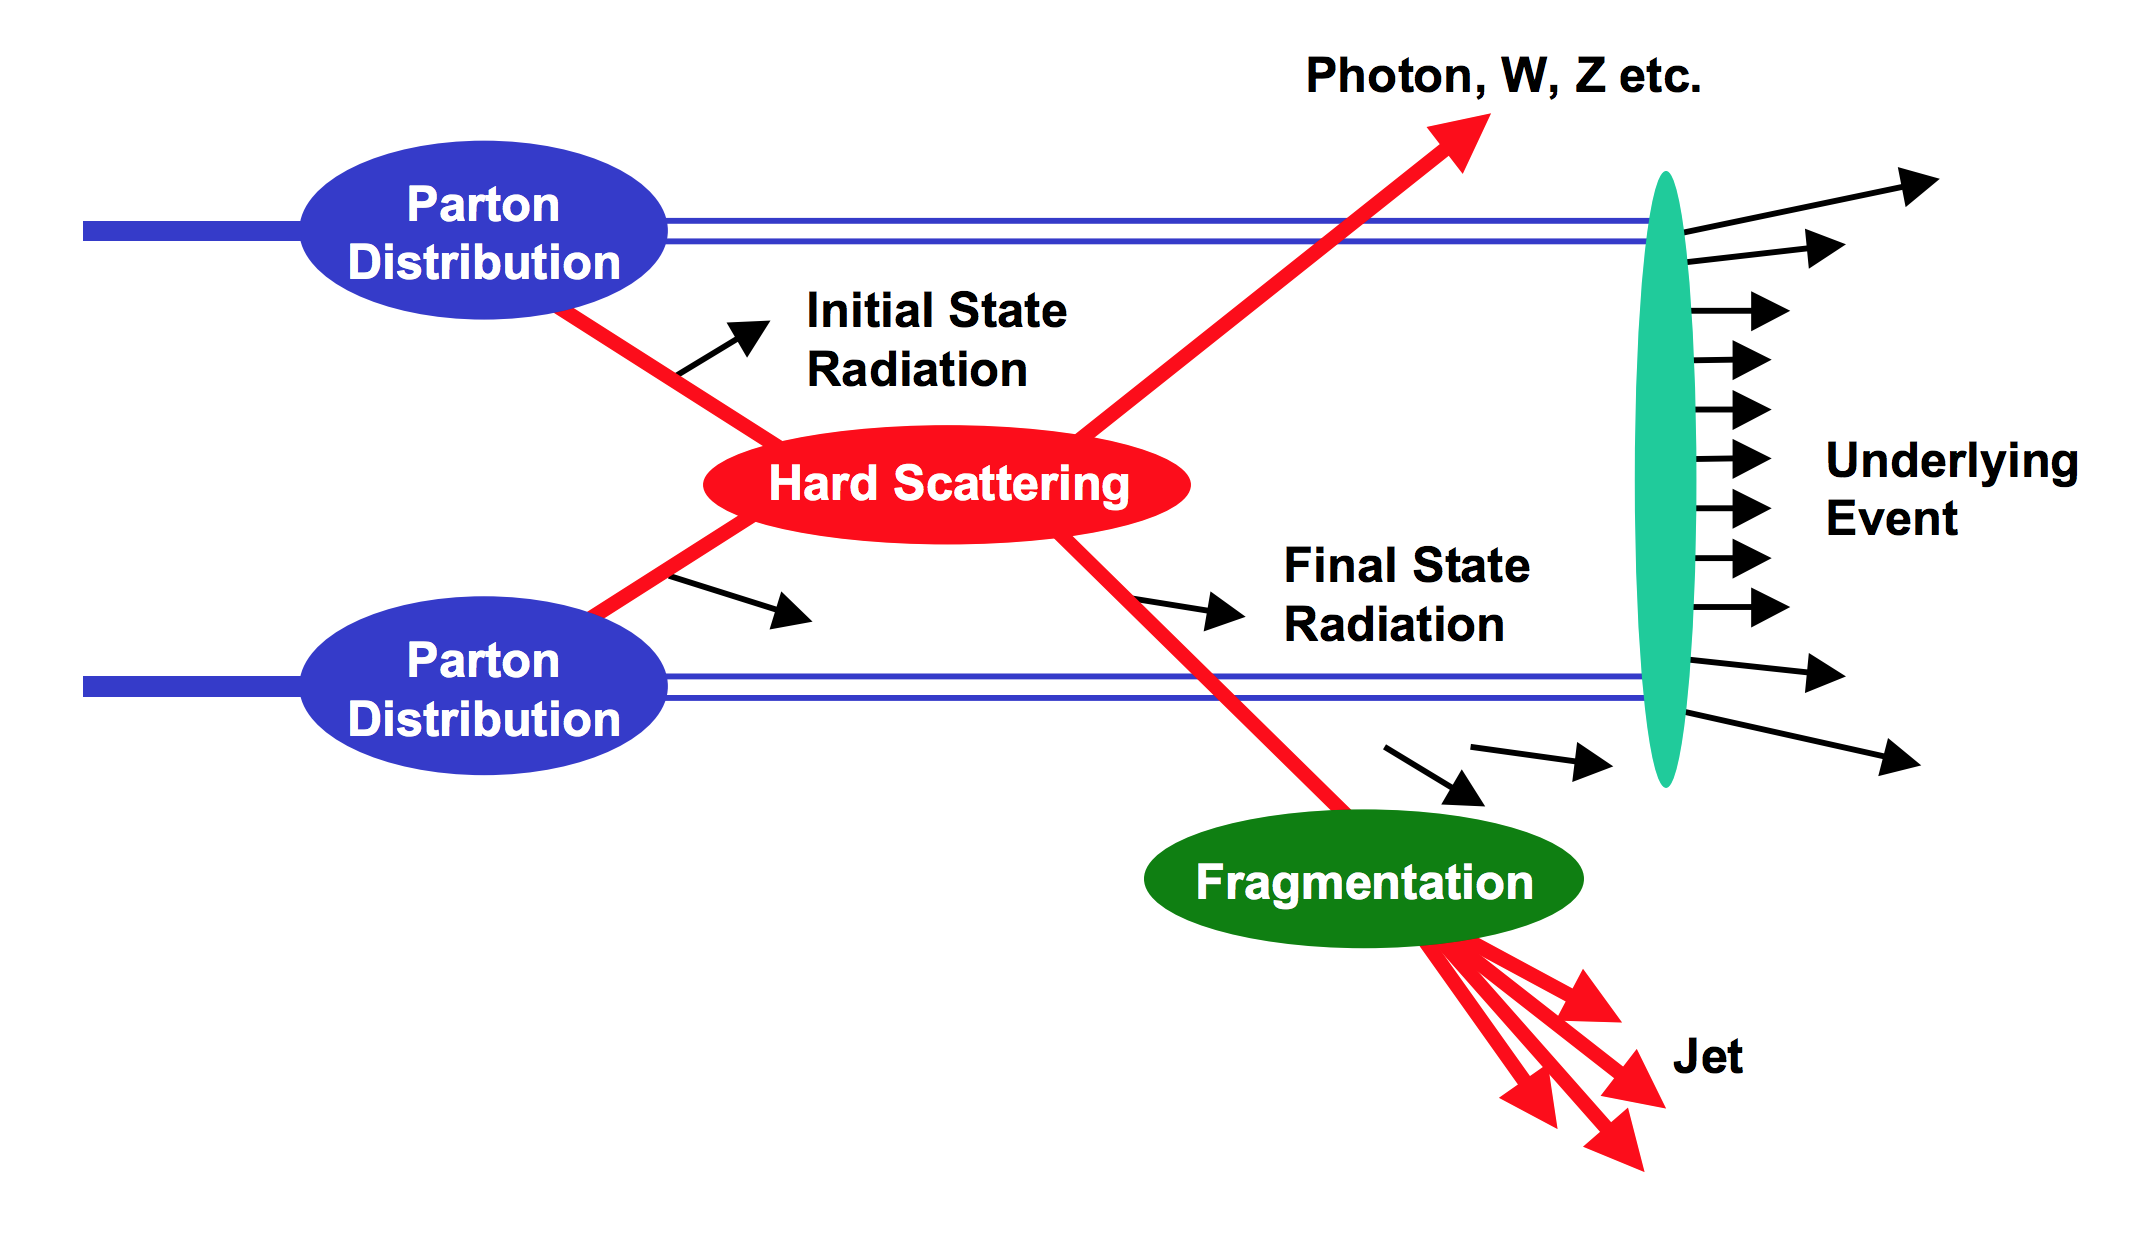
\includegraphics[width=0.7\textwidth]{figures/Theory/hh_collision.png}
  \caption{Schematic view of a hadron-hadron collision \cite{Womersley:2000cx}.}
  \label{fig:C2_had_col}
\end{figure}
and the typical features are summarized as below:
\begin{itemize}
	\item \textbf{Parton Distribution Function (PDF)}: $f_{i}\left(x, Q^{2}\right)$ gives the probability of a parton with flavor $i$ (quark or gluon), carrying a momentum fraction of $x$ and at the energy of Q in a proton. Parton distribution function cannot be fully calculated by perturbative QCD because of the inherent non-perturbative nature of partons. There are many different sets of PDFs that are determined by a fit to data from experimental observables in various processes. As an example, figure~\ref{fig:C2_PDF4LHC15} shows the \textit{PDF4LHC15 NLO PDFs}, which is based on the combination of the \textit{CT14}, \textit{MMHT14} and \textit{NNPDF3.1} NNLO PDF sets \cite{Lin:2017snn}.
	\item \textbf{Fragmentation and hadronization}: The processes to produce final state particles (or jets) from the partons produced in hard scattering.
	\item \textbf{Initial/Final state radiation}: The incoming and outgoing partons that carry color charge can emit QCD radiation, which gives rise to additional jets. Also the charged incoming and outgoing particles can emit Quantum Electrodynamics (QED) radiations with photons.
	\item \textbf{Underlying events}: Products from soft processes (not come from the primary hard scattering) as the remnants of scattering interactions.
\end{itemize}
\begin{figure}[!htb]
  \centering
  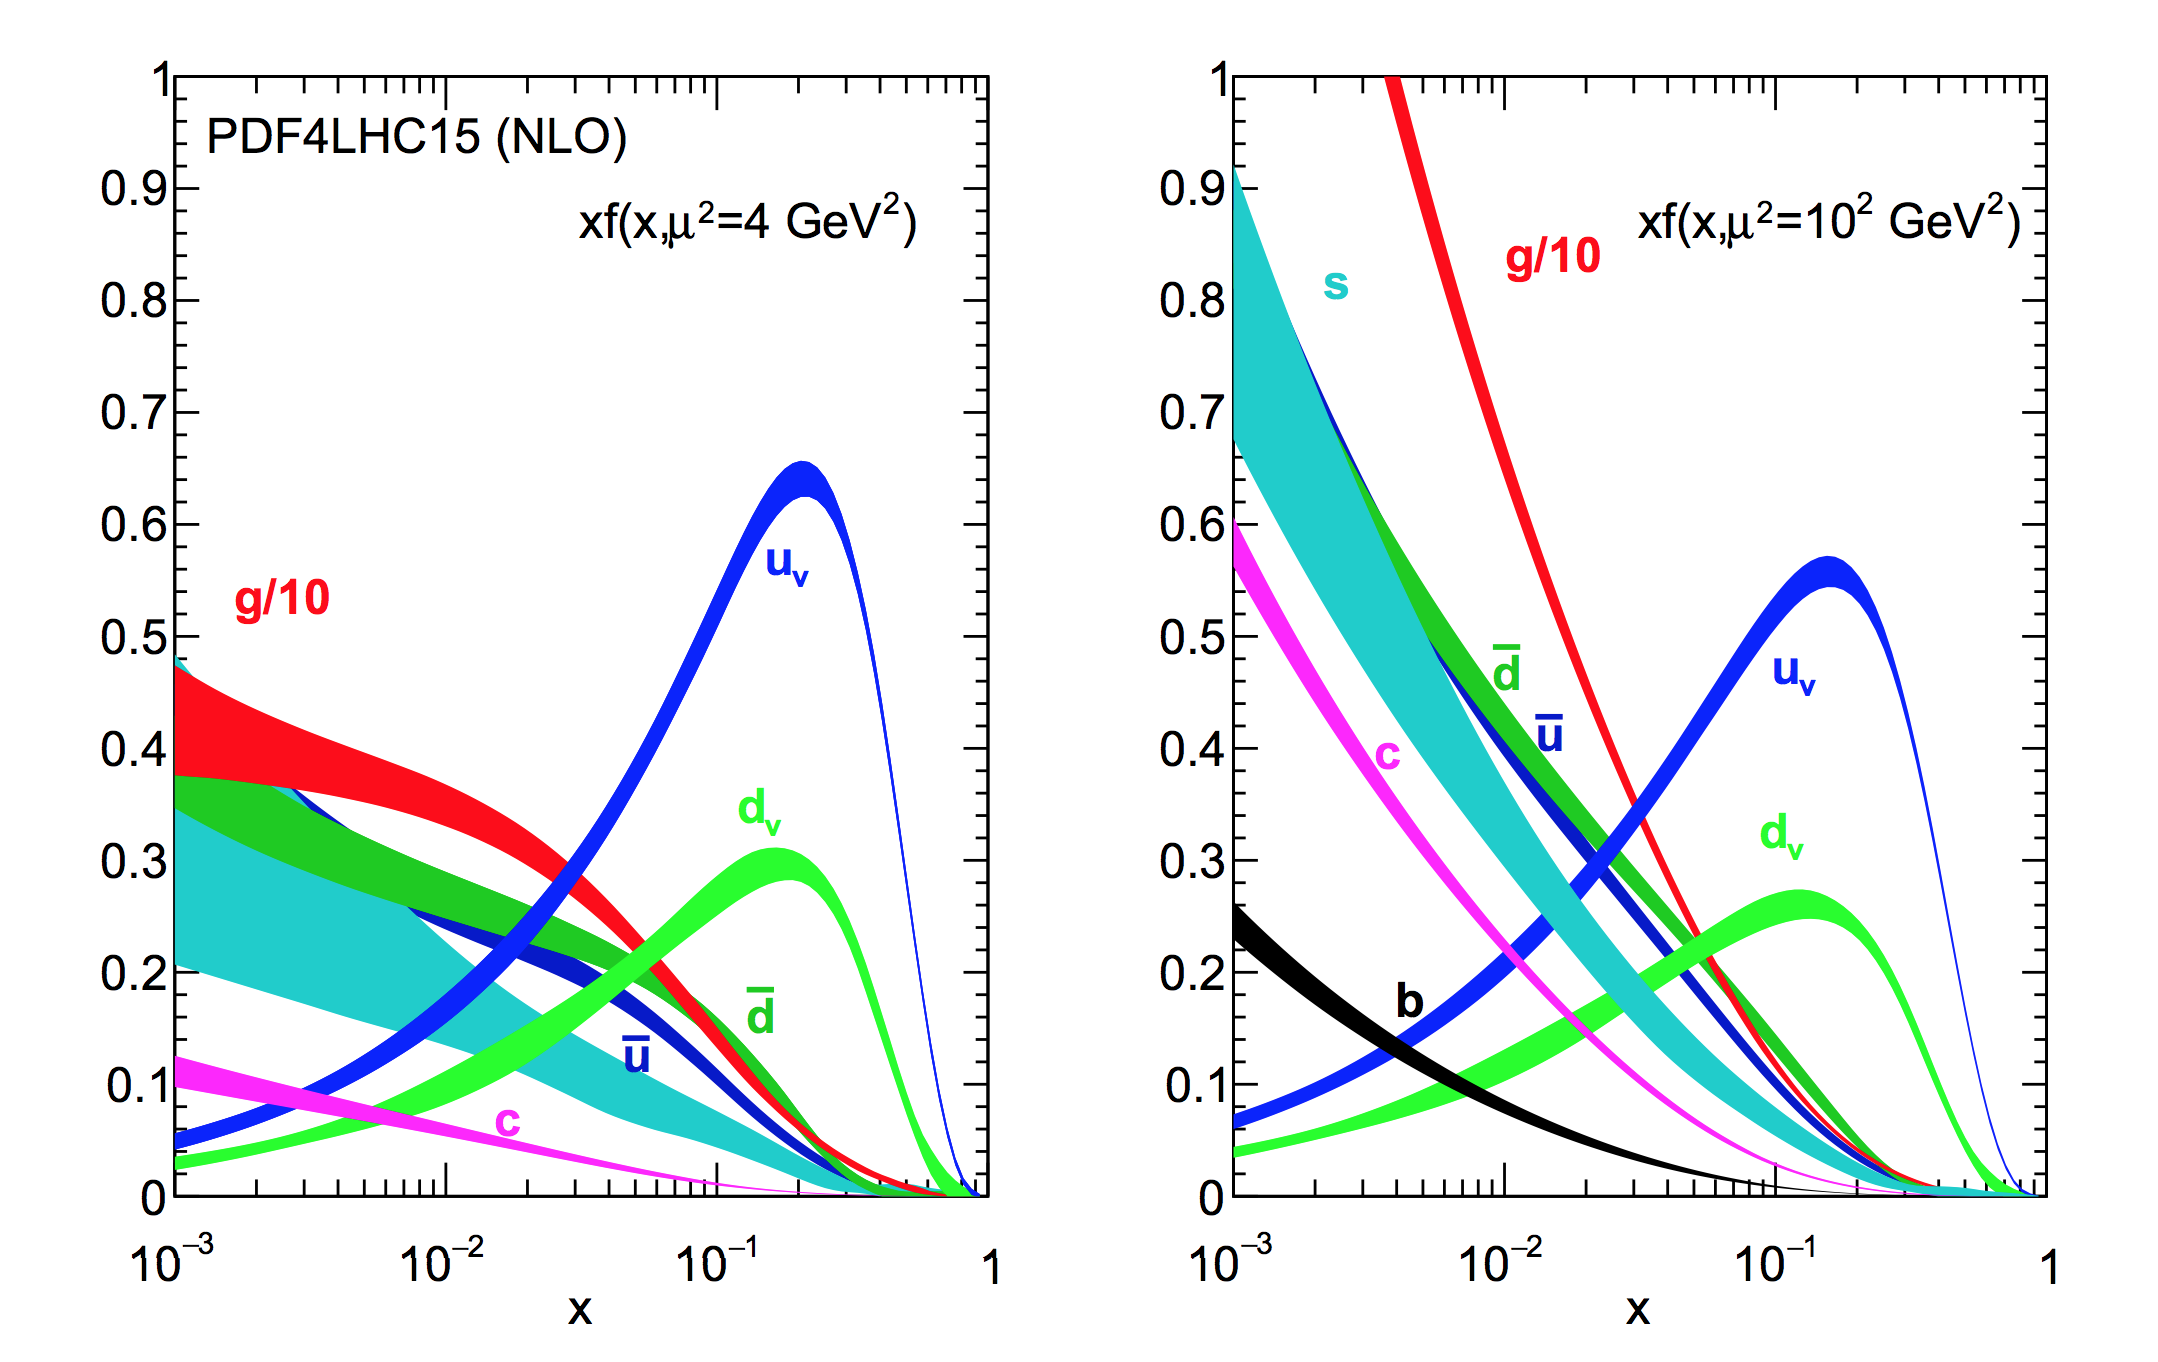
\includegraphics[width=0.7\textwidth]{figures/Theory/PDF4LHC15.png}
  \caption{The PDF4LHC15 NLO PDFs at a low scale $\mu^{2} = Q^{2} = 4 GeV^{2}$ (left) and at $\mu^{2} = Q^{2} = 100 GeV^{2}$ (right) as a function of x.}
  \label{fig:C2_PDF4LHC15}
\end{figure}

\textbf{Cross section of hard scaterring} 

According to \textit{QCD factorization theorems} \cite{Collins:1989gx}, the perturbative calculations can be applied to many important
hard processes involving hadrons. The basic problem addressed by factorization theorems is how to calculate high energy cross sections.
Consider the process of scattering between two hardons A and B to produce a final state X, the cross section $\sigma$ can be obtained 
by summing over all the subprocess cross section $\hat{\sigma}$ \cite{Stirling:1194745}
\begin{equation}
	\sigma_{AB} = \int dx_{a} dx_{b} f_{a/A}\left(x_{a}\right) f_{b/B}\left(x_{b}\right) \hat{\sigma}_{ab\rightarrow X}
\end{equation}
where $f_{q/A}\left(x_{q}\right)$ is the parton distribution functions of parton $q$.
Taking into account the leading order correction:
\begin{equation} \label{eq:xs2}
	\sigma_{AB} = \int dx_{a} dx_{b} f_{a/A}\left(x_{a}Q^{2}\right) f_{b/B}\left(x_{b}Q^{2}\right) \hat{\sigma}_{ab\rightarrow X}
\end{equation}
where $Q^{2}$ represents large momentum scale that characterizes the hard scattering.
Later on, since the finite corrections were not universal and had to be calculated separately for each process,
the perturbative $O\left(\alpha_{S}^{n}\right)$ corrections to the leading logarithm cross section in Eq.~\ref{eq:xs2}
need to be applied, one can get:
\begin{equation}
	\sigma_{AB} = \int dx_{a} dx_{b} f_{a/A}\left(x_{a}\mu_{F}^{2}\right) f_{b/B}\left(x_{b}\mu_{F}^{2}\right) \hat{\sigma}_{ab\rightarrow X}\left(\alpha_{S},\mu_{R},\mu_{F}\right)
\end{equation}
in which $\mu_{F}$ is \textit{factorization scale} which can represent the scale that separates the long- and short-distance physics,
and $\mu_{R}$ is the \textit{renormalization scale} for QCD running coupling.
$\hat{\sigma}_{ab\rightarrow X}$ is the parton-level hard scattering cross section that can be calculated perturbatively in QCD with the form of
\begin{equation} \label{eq:xs3}
	\hat{\sigma}_{ab\rightarrow X}\left(\alpha_{S},\mu_{R},\mu_{F}\right) 
		= \left(\alpha_{S}\right)^{n} \left[ \hat{\sigma}^{(0)}
		+ \left(\alpha_{S}/2\pi\right) \hat{\sigma}^{(1)}\left(\mu_{R},\mu_{F}\right)
		+ \left(\alpha_{S}/2\pi\right)^{2} \hat{\sigma}^{(2)}\left(\mu_{R},\mu_{F}\right)
		+ ... \right]
\end{equation}
where $\hat{\sigma}^{(0)}$ stands for the leading-order (LO) partonic cross section,
while $\hat{\sigma}^{(1)}$ and $\hat{\sigma}^{(2)}$ are the next-to-leading-order (NLO) and
next-to-next-to-leading-order (NNLO) cross section.

$\mu_{R}$ and $\mu_{F}$ depend on the order of truncation in Eq.~\ref{eq:xs3}.
In principle, if cross section is calculated to all orders, it is invariant under changes in these parameters.
The choices of $\mu_{R}$ and $\mu_{F}$ are arbitrary. 
To avoid unnaturally large logarithms reappearing in the perturbation series,
it is sensible to choose $\mu_{R}$ and $\mu_{F}$ values of the order of the typical momentum scales of
the hard scattering process and $\mu_{R} = \mu_{F}$ is also often assumed.
Take Drell–Yan process as an example, the standard choice is $\mu_{R} = \mu_{F} = m_{ll}$, 
where $m_{ll}$ is the invariant mass of di-lepton pair.
